\begin{frame}{Large Language Models}
   \begin{columns}
         
       \begin{column}[t]{0.4\textwidth}
       \begin{block}{Summary}
       
           \begin{itemize}
               \item State-of-the-art of Natural Language Processing (NLP) problems
               \item Architecture : Transformers\footnote{Vaswani et al, Attention is all you need,2017} block, mixed with classical layers (MLP, Conv)
           \end{itemize}
               
   
       \end{block}
       \end{column}
           
       \begin{column}[t]{0.55\textwidth}
       \begin{block}{Self Attention }
   
           \begin{figure}
               \centering
               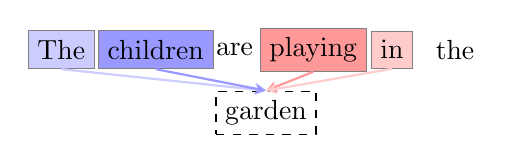
\begin{tikzpicture}[node distance=0.8cm]

    % Define block styles
    \tikzstyle{model} = [rectangle,rounded corners, minimum width=2cm, minimum height=1cm, text centered, draw=black, fill=blue!30]
    \tikzstyle{arrow} = [thick,->,>=stealth]
    
    % Define nodes
    \node (the) [fill=blue!20,rectangle,draw=black!50] {The};
    \node (children) [right of = the,fill=blue!40,rectangle,draw=black!50,xshift=0.4cm] {children};
    \node (are) [right of = children,xshift=0.2cm] {are};
    \node (playing) [right of = are,fill=red!40,rectangle,draw=black!50,xshift=0.2cm] {playing};
    \node (in) [right of = playing,fill=red!20,rectangle,draw=black!50,xshift=0.2cm] {in};
    \node (the2) [right of = in] {the};
    
    \node (garden) [below of = are, xshift=0.4cm,rectangle,dashed,draw=black] {garden};
    
    % Draw arrows
    \draw [arrow,draw=blue!20] (the.south) -- (garden.north);
    \draw [arrow,draw=blue!40] (children.south) -- (garden.north);
    \draw [arrow,draw=red!40] (playing.south) -- (garden.north);
    \draw [arrow,draw=red!20] (in.south) -- (garden.north);
    
    % Add a rectangle around the last four nodes
    \end{tikzpicture}
               \caption{Self Attention mecanism illustration}
           \end{figure}
       
           Self attention is the key of LLM, used to compute the context of each token.
       \end{block}  
       \end{column}
            
   \end{columns}
   \end{frame}

\begin{frame}{Fine Tuning}
   
\end{frame}

\begin{frame}{Hyperparameter Optimization}
   
\end{frame}

\begin{frame}{Problem Formulation}
   
\end{frame}

\begin{frame}{Related Works}
   
\end{frame}